\documentclass[]{article}
\usepackage{lmodern}
\usepackage{amssymb,amsmath}
\usepackage{ifxetex,ifluatex}
\usepackage{fixltx2e} % provides \textsubscript
\ifnum 0\ifxetex 1\fi\ifluatex 1\fi=0 % if pdftex
  \usepackage[T1]{fontenc}
  \usepackage[utf8]{inputenc}
\else % if luatex or xelatex
  \ifxetex
    \usepackage{mathspec}
  \else
    \usepackage{fontspec}
  \fi
  \defaultfontfeatures{Ligatures=TeX,Scale=MatchLowercase}
\fi
% use upquote if available, for straight quotes in verbatim environments
\IfFileExists{upquote.sty}{\usepackage{upquote}}{}
% use microtype if available
\IfFileExists{microtype.sty}{%
\usepackage{microtype}
\UseMicrotypeSet[protrusion]{basicmath} % disable protrusion for tt fonts
}{}
\usepackage[margin=1in]{geometry}
\usepackage{hyperref}
\hypersetup{unicode=true,
            pdftitle={TP2 de Statistique},
            pdfauthor={Nicolas Makaroff},
            pdfborder={0 0 0},
            breaklinks=true}
\urlstyle{same}  % don't use monospace font for urls
\usepackage{color}
\usepackage{fancyvrb}
\newcommand{\VerbBar}{|}
\newcommand{\VERB}{\Verb[commandchars=\\\{\}]}
\DefineVerbatimEnvironment{Highlighting}{Verbatim}{commandchars=\\\{\}}
% Add ',fontsize=\small' for more characters per line
\usepackage{framed}
\definecolor{shadecolor}{RGB}{248,248,248}
\newenvironment{Shaded}{\begin{snugshade}}{\end{snugshade}}
\newcommand{\AlertTok}[1]{\textcolor[rgb]{0.94,0.16,0.16}{#1}}
\newcommand{\AnnotationTok}[1]{\textcolor[rgb]{0.56,0.35,0.01}{\textbf{\textit{#1}}}}
\newcommand{\AttributeTok}[1]{\textcolor[rgb]{0.77,0.63,0.00}{#1}}
\newcommand{\BaseNTok}[1]{\textcolor[rgb]{0.00,0.00,0.81}{#1}}
\newcommand{\BuiltInTok}[1]{#1}
\newcommand{\CharTok}[1]{\textcolor[rgb]{0.31,0.60,0.02}{#1}}
\newcommand{\CommentTok}[1]{\textcolor[rgb]{0.56,0.35,0.01}{\textit{#1}}}
\newcommand{\CommentVarTok}[1]{\textcolor[rgb]{0.56,0.35,0.01}{\textbf{\textit{#1}}}}
\newcommand{\ConstantTok}[1]{\textcolor[rgb]{0.00,0.00,0.00}{#1}}
\newcommand{\ControlFlowTok}[1]{\textcolor[rgb]{0.13,0.29,0.53}{\textbf{#1}}}
\newcommand{\DataTypeTok}[1]{\textcolor[rgb]{0.13,0.29,0.53}{#1}}
\newcommand{\DecValTok}[1]{\textcolor[rgb]{0.00,0.00,0.81}{#1}}
\newcommand{\DocumentationTok}[1]{\textcolor[rgb]{0.56,0.35,0.01}{\textbf{\textit{#1}}}}
\newcommand{\ErrorTok}[1]{\textcolor[rgb]{0.64,0.00,0.00}{\textbf{#1}}}
\newcommand{\ExtensionTok}[1]{#1}
\newcommand{\FloatTok}[1]{\textcolor[rgb]{0.00,0.00,0.81}{#1}}
\newcommand{\FunctionTok}[1]{\textcolor[rgb]{0.00,0.00,0.00}{#1}}
\newcommand{\ImportTok}[1]{#1}
\newcommand{\InformationTok}[1]{\textcolor[rgb]{0.56,0.35,0.01}{\textbf{\textit{#1}}}}
\newcommand{\KeywordTok}[1]{\textcolor[rgb]{0.13,0.29,0.53}{\textbf{#1}}}
\newcommand{\NormalTok}[1]{#1}
\newcommand{\OperatorTok}[1]{\textcolor[rgb]{0.81,0.36,0.00}{\textbf{#1}}}
\newcommand{\OtherTok}[1]{\textcolor[rgb]{0.56,0.35,0.01}{#1}}
\newcommand{\PreprocessorTok}[1]{\textcolor[rgb]{0.56,0.35,0.01}{\textit{#1}}}
\newcommand{\RegionMarkerTok}[1]{#1}
\newcommand{\SpecialCharTok}[1]{\textcolor[rgb]{0.00,0.00,0.00}{#1}}
\newcommand{\SpecialStringTok}[1]{\textcolor[rgb]{0.31,0.60,0.02}{#1}}
\newcommand{\StringTok}[1]{\textcolor[rgb]{0.31,0.60,0.02}{#1}}
\newcommand{\VariableTok}[1]{\textcolor[rgb]{0.00,0.00,0.00}{#1}}
\newcommand{\VerbatimStringTok}[1]{\textcolor[rgb]{0.31,0.60,0.02}{#1}}
\newcommand{\WarningTok}[1]{\textcolor[rgb]{0.56,0.35,0.01}{\textbf{\textit{#1}}}}
\usepackage{graphicx,grffile}
\makeatletter
\def\maxwidth{\ifdim\Gin@nat@width>\linewidth\linewidth\else\Gin@nat@width\fi}
\def\maxheight{\ifdim\Gin@nat@height>\textheight\textheight\else\Gin@nat@height\fi}
\makeatother
% Scale images if necessary, so that they will not overflow the page
% margins by default, and it is still possible to overwrite the defaults
% using explicit options in \includegraphics[width, height, ...]{}
\setkeys{Gin}{width=\maxwidth,height=\maxheight,keepaspectratio}
\IfFileExists{parskip.sty}{%
\usepackage{parskip}
}{% else
\setlength{\parindent}{0pt}
\setlength{\parskip}{6pt plus 2pt minus 1pt}
}
\setlength{\emergencystretch}{3em}  % prevent overfull lines
\providecommand{\tightlist}{%
  \setlength{\itemsep}{0pt}\setlength{\parskip}{0pt}}
\setcounter{secnumdepth}{0}
% Redefines (sub)paragraphs to behave more like sections
\ifx\paragraph\undefined\else
\let\oldparagraph\paragraph
\renewcommand{\paragraph}[1]{\oldparagraph{#1}\mbox{}}
\fi
\ifx\subparagraph\undefined\else
\let\oldsubparagraph\subparagraph
\renewcommand{\subparagraph}[1]{\oldsubparagraph{#1}\mbox{}}
\fi

%%% Use protect on footnotes to avoid problems with footnotes in titles
\let\rmarkdownfootnote\footnote%
\def\footnote{\protect\rmarkdownfootnote}

%%% Change title format to be more compact
\usepackage{titling}

% Create subtitle command for use in maketitle
\newcommand{\subtitle}[1]{
  \posttitle{
    \begin{center}\large#1\end{center}
    }
}

\setlength{\droptitle}{-2em}

  \title{TP2 de Statistique}
    \pretitle{\vspace{\droptitle}\centering\huge}
  \posttitle{\par}
    \author{Nicolas Makaroff}
    \preauthor{\centering\large\emph}
  \postauthor{\par}
      \predate{\centering\large\emph}
  \postdate{\par}
    \date{01/03/2019}


\begin{document}
\maketitle

\#1 - Théorème Central Limite et Estimation de Monte Carlo \#\#\#
Avant-propos

Pour la suite de l'exercice, on définit trois fonctions permettant d'une
part pour un vecteur donné de calculer la moyenne empirique et la
variance empirique, et d'autre part pour une loi donné de créer un
échantillon de taille \(N=1000\).

\begin{Shaded}
\begin{Highlighting}[]
\NormalTok{N<-}\DecValTok{1000}
\NormalTok{n<-}\KeywordTok{c}\NormalTok{(}\DecValTok{5}\NormalTok{,}\DecValTok{30}\NormalTok{,}\DecValTok{100}\NormalTok{)}
\CommentTok{#Fonction calculant la moyenne empirique pour un vecteur donné}
\NormalTok{moy_empirique <-}\StringTok{ }\ControlFlowTok{function}\NormalTok{(vecteur)\{}
\NormalTok{ sum<-}\DecValTok{0}
 \ControlFlowTok{for}\NormalTok{ (i }\ControlFlowTok{in}\NormalTok{ vecteur)\{}
\NormalTok{   sum<-sum }\OperatorTok{+}\StringTok{ }\NormalTok{i}
\NormalTok{ \}}
 \KeywordTok{return}\NormalTok{ (sum}\OperatorTok{/}\NormalTok{(}\KeywordTok{length}\NormalTok{(vecteur)))}
\NormalTok{\}}

\CommentTok{#Calcul de la variance emmpirique pour un vecteur donné}
\NormalTok{var_empirique <-}\StringTok{ }\ControlFlowTok{function}\NormalTok{(vecteur)\{}
\NormalTok{  moy<-}\KeywordTok{moy_empirique}\NormalTok{(vecteur)}
\NormalTok{  sum<-}\DecValTok{0}
  \ControlFlowTok{for}\NormalTok{ (i }\ControlFlowTok{in}\NormalTok{ vecteur)\{}
\NormalTok{    sum <-}\StringTok{ }\NormalTok{sum  }\OperatorTok{+}\StringTok{ }\NormalTok{(i}\OperatorTok{-}\NormalTok{moy)}\OperatorTok{*}\NormalTok{(i}\OperatorTok{-}\NormalTok{moy)}
\NormalTok{  \}}
  \KeywordTok{return}\NormalTok{ ( sum}\OperatorTok{/}\NormalTok{(}\KeywordTok{length}\NormalTok{(vecteur)}\OperatorTok{-}\DecValTok{1}\NormalTok{))}
\NormalTok{\}}
\end{Highlighting}
\end{Shaded}

On introduit aussi une fonction permettant de calculer la moyenne
empirique sur un échantillon en fonction de n'importe quelle loi et
compare avec la loi normale.

\#\#\#1.1 Simulation de 1000 échantillon i.i.d Gaussien

\begin{Shaded}
\begin{Highlighting}[]
\NormalTok{gen_echan_gauss <-}\StringTok{ }\ControlFlowTok{function}\NormalTok{(n,N,mu,sigma)\{}
\NormalTok{    x <-}\StringTok{ }\KeywordTok{rnorm}\NormalTok{(n,mu,sigma)}
\NormalTok{    aleatoire <-}\StringTok{ }\ControlFlowTok{function}\NormalTok{(x1,n1)\{}
\NormalTok{      y <-}\StringTok{ }\KeywordTok{sample}\NormalTok{(x1,n1,}\DataTypeTok{replace=}\OtherTok{TRUE}\NormalTok{)}
\NormalTok{      moy_sd <-}\StringTok{ }\KeywordTok{c}\NormalTok{(}\KeywordTok{moy_empirique}\NormalTok{(y),}\KeywordTok{var_empirique}\NormalTok{(y))}
     \KeywordTok{return}\NormalTok{(moy_sd)}
\NormalTok{    \}}
\NormalTok{  result <-}\StringTok{ }\KeywordTok{sapply}\NormalTok{(}\DecValTok{1}\OperatorTok{:}\NormalTok{N,}\ControlFlowTok{function}\NormalTok{(w) }\KeywordTok{aleatoire}\NormalTok{(x,n))}
  
  \KeywordTok{return}\NormalTok{(result)}
\NormalTok{\}}
\NormalTok{hist_mul <-}\StringTok{ }\ControlFlowTok{function}\NormalTok{(n)\{}
  \ControlFlowTok{for}\NormalTok{ (i }\ControlFlowTok{in}\NormalTok{ n)\{}
    \KeywordTok{hist}\NormalTok{(}\KeywordTok{gen_echan_gauss}\NormalTok{(i,N,}\DecValTok{1}\NormalTok{,}\DecValTok{2}\NormalTok{)[}\DecValTok{1}\NormalTok{,],}\DataTypeTok{breaks=}\NormalTok{i)}
\NormalTok{    t <-}\StringTok{ }\KeywordTok{seq}\NormalTok{(}\OperatorTok{-}\DecValTok{10}\NormalTok{,}\DecValTok{10}\NormalTok{,}\DataTypeTok{by=}\FloatTok{0.5}\NormalTok{)}
\NormalTok{x <-}\StringTok{ }\KeywordTok{dnorm}\NormalTok{(t,}\DecValTok{1}\NormalTok{,}\DecValTok{2}\NormalTok{)}
\KeywordTok{par}\NormalTok{(}\DataTypeTok{new=}\OtherTok{TRUE}\NormalTok{)}
\CommentTok{#plot(x)}
\KeywordTok{curve}\NormalTok{(}\KeywordTok{dnorm}\NormalTok{(x,}\DecValTok{1}\NormalTok{,}\DecValTok{2}\NormalTok{),}\OperatorTok{-}\DecValTok{5}\NormalTok{,}\DecValTok{5}\NormalTok{)}
\NormalTok{  \}}
\NormalTok{\}}
\CommentTok{#hist_moy(function(n)\{return (rnorm(n,mean=1,sd=2))\},"Distribution Gausienne N(1,2)")}
\KeywordTok{hist_mul}\NormalTok{(n)}
\end{Highlighting}
\end{Shaded}

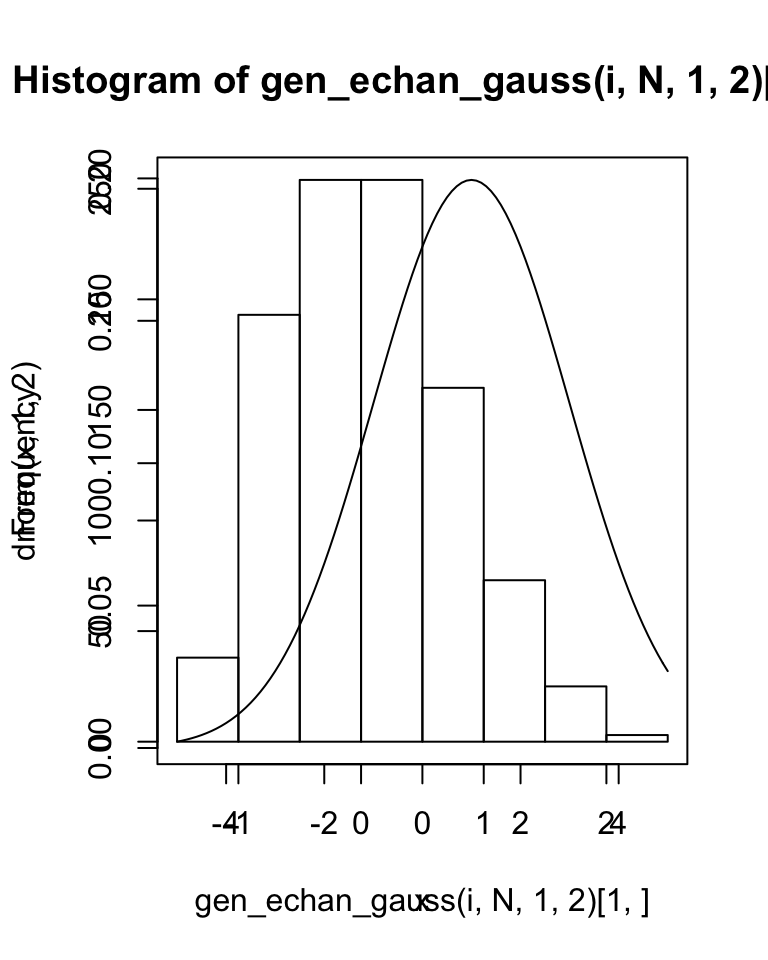
\includegraphics{tp2_files/figure-latex/unnamed-chunk-2-1.pdf}
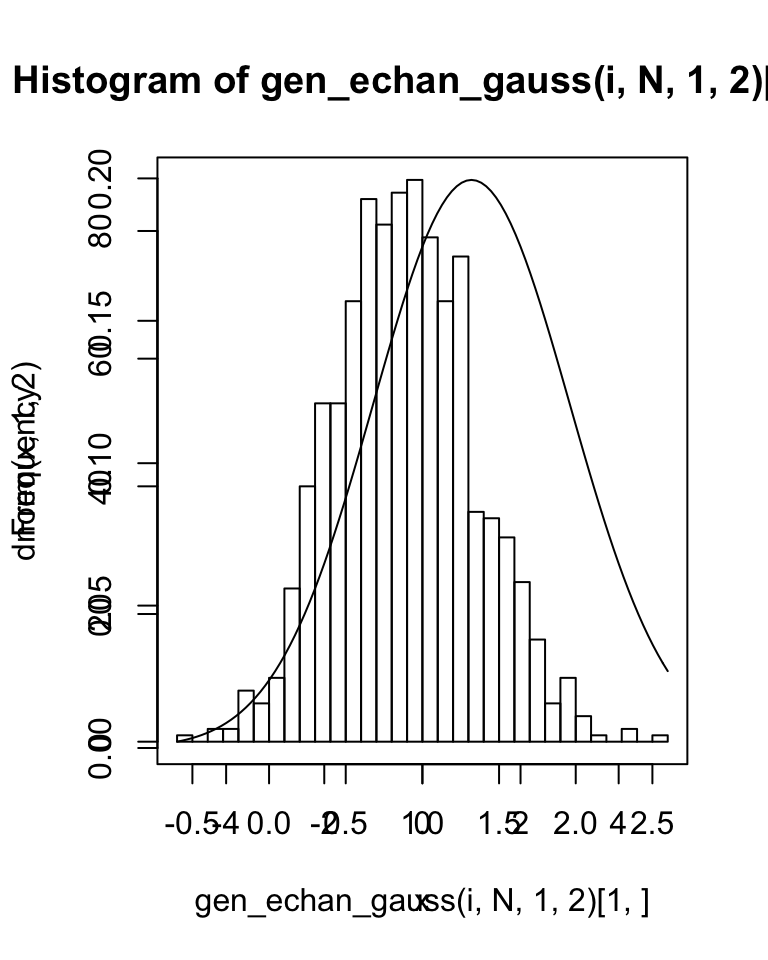
\includegraphics{tp2_files/figure-latex/unnamed-chunk-2-2.pdf}
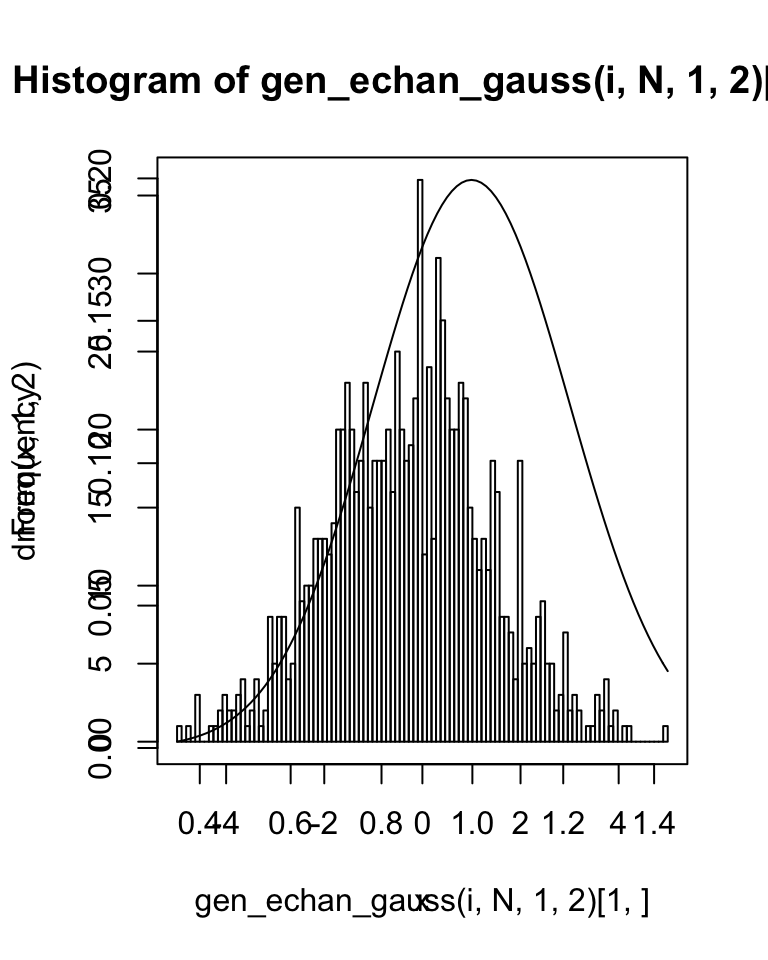
\includegraphics{tp2_files/figure-latex/unnamed-chunk-2-3.pdf}

Soit \(S_{n}=\sum\limits_{i=1}^{n}X_{i}\) tq : \(X_{i}\) i.i.d en loi de
moyenne \(\mu\) et variance \(\sigma^{2}\).

D'après le théorème centrale limite, comme \(N\) est assez grand, on en
déduit que \(S_{n}\) peut être approchée une loi normal
\(\mathcal{N}(n\mu,n\sigma^{2})\).

On pose : \({X_{n}} = \frac{S_{n}}{n}\) Ainsi, pour la moyenne :
\(\mathbb{E}[ X_{n}]=\mathbb{E}[\frac{S_{n}}{n}]=\frac{1}{n}\mathbb{E}[S_{n}]=\frac{1}{n}\sum\limits_{i=0}^{n}\mathbb{E}[X_{i}]=\mathbb{E}[X_{i}]\)
De même pour la variance :
\(\mathbb{V}[{ X_{n}}]=\mathbb{V}[\frac{S_{n}}{n}]=\frac{1}{n^{2}}\mathbb{V}[S_{n}]=\frac{1}{n^{2}}\sum\limits_{i=0}^{n}\mathbb{V}[X_{i}]=\frac{1}{n}\mathbb{V}[X_{i}]\)

Dans le cas de la question 1. on a : \(\mathcal{N}(1,2)\) On note, avec
les notations de l'énoncé,
\((a_{n},b_{n})=(\mathbb{E}[X_i],\sqrt{\frac{1}{n}\mathbb{V}[Xi]})=(\mu,\sqrt\frac{\sigma^{2}}{n})\)
Ce qui donne pour le cas présent : \((1,\frac{2}{\sqrt{n}})\)

Ainsi, on en déduit que \(U_{n}=\frac{{X_{n}} - a_{n}}{b_{n}}\) suit une
loi normale centrée réduite \(\mathcal{N}(0,1)\).

\begin{Shaded}
\begin{Highlighting}[]
\CommentTok{#Fonction que trace l'histogramme pour la loi centrée réduite. Pour varier, j'ai utilisé ici une autre manière de créer un échantillon.}
\NormalTok{moy_norm_hist <-}\StringTok{ }\ControlFlowTok{function}\NormalTok{(law,title)\{}
  \ControlFlowTok{for}\NormalTok{ (j }\ControlFlowTok{in}\NormalTok{ n)\{}
\NormalTok{    sample <-}\KeywordTok{law}\NormalTok{(j}\OperatorTok{*}\NormalTok{N)}
\NormalTok{    Xn <-}\StringTok{ }\KeywordTok{moy_empirique}\NormalTok{(sample)}
\NormalTok{    Un <-}\StringTok{ }\KeywordTok{c}\NormalTok{()}
    \ControlFlowTok{for}\NormalTok{ (i }\ControlFlowTok{in} \DecValTok{1}\OperatorTok{:}\NormalTok{N)\{}
\NormalTok{      sample2 <-}\StringTok{ }\NormalTok{sample[((i}\DecValTok{-1}\NormalTok{)}\OperatorTok{*}\NormalTok{j }\OperatorTok{+}\StringTok{ }\DecValTok{1}\NormalTok{)}\OperatorTok{:}\StringTok{ }\NormalTok{(i}\OperatorTok{*}\NormalTok{j)]}
\NormalTok{      ani <-}\StringTok{ }\KeywordTok{moy_empirique}\NormalTok{(sample2)}
\NormalTok{      bni <-}\StringTok{ }\KeywordTok{var_empirique}\NormalTok{(sample2) }\OperatorTok{/}\StringTok{ }\KeywordTok{sqrt}\NormalTok{(j)}
\NormalTok{      Uni <-}\StringTok{ }\NormalTok{(Xn }\OperatorTok{-}\StringTok{ }\NormalTok{ani)}\OperatorTok{/}\StringTok{ }\NormalTok{bni}
\NormalTok{      Un <-}\StringTok{ }\KeywordTok{c}\NormalTok{(Un,Uni)}
\NormalTok{    \}}
    \KeywordTok{hist}\NormalTok{(Un, }\DataTypeTok{xlab=}\KeywordTok{paste}\NormalTok{(}\StringTok{"Moyenne empirique centrée réduite pour une taille="}\NormalTok{,j),}\DataTypeTok{main=}\NormalTok{title,}\DataTypeTok{breaks=}\NormalTok{j)}
\NormalTok{  \}}
\NormalTok{\}}
\KeywordTok{mean}\NormalTok{(}\KeywordTok{gen_echan_gauss}\NormalTok{(}\DecValTok{100}\NormalTok{,}\DecValTok{1000}\NormalTok{,}\DecValTok{1}\NormalTok{,}\DecValTok{2}\NormalTok{))}
\end{Highlighting}
\end{Shaded}

\begin{verbatim}
## [1] 2.269809
\end{verbatim}

\begin{Shaded}
\begin{Highlighting}[]
\CommentTok{#moy_empirique(gen_echan_gauss(10000,10000,1,2))}
\NormalTok{moy_norm <-}\StringTok{ }\ControlFlowTok{function}\NormalTok{(n,N,mu,sigma)\{}
\NormalTok{  Xn <-}\StringTok{ }\KeywordTok{gen_echan_gauss}\NormalTok{(n,N,mu,sigma)[}\DecValTok{1}\NormalTok{,]}
\NormalTok{  Un <-}\StringTok{ }\KeywordTok{c}\NormalTok{()}
  \ControlFlowTok{for}\NormalTok{ (i }\ControlFlowTok{in}\NormalTok{ Xn)\{}
\NormalTok{    an <-}\StringTok{ }\NormalTok{mu}
\NormalTok{    bn <-}\StringTok{ }\KeywordTok{sqrt}\NormalTok{(sigma}\OperatorTok{*}\NormalTok{sigma}\OperatorTok{/}\NormalTok{n)}
\NormalTok{    Un <-}\StringTok{ }\KeywordTok{c}\NormalTok{(Un,(i}\OperatorTok{-}\NormalTok{an)}\OperatorTok{/}\NormalTok{bn)}
\NormalTok{  \}}
  \KeywordTok{return}\NormalTok{(Un)}
\NormalTok{\}}
\CommentTok{#hist(moy_norm(1000,10000,1,2),breaks=100)}
\CommentTok{#moy_norm_hist(function(n) \{return (rnorm(n , mean=1, sd=2))\},"Distribution gaussienne N(1,2)")}
\CommentTok{#t <- seq(-10,10,by=0.5)}
\CommentTok{#x <- dnorm(t)}
\CommentTok{#par(new=TRUE)}
\CommentTok{#curve(dnorm(x),-3,3)}
\end{Highlighting}
\end{Shaded}

On obtient bien une loi centrée reduite. On remarque que plus n est
grand plus la loi suivi ce rapproche de la loi centré réduite.

\#\#\#1.2 Loi de Pareto

Soit \(X\) une variable aléatoire suivant une loi de Pareto
\(\mathcal{P}(a, \alpha)\),où \(\alpha > 2\). Alors,
\(\mathbb{E}[X]=\frac{\alpha \times a}{\alpha - 1}\) et
\(\mathbb{V}[X]=(\frac{\alpha \times a}{\alpha - 1})^2\frac{\alpha}{\alpha - 2}\)
On cherche encore une fois à appliquer le théorème centrale limite afin
de mettre en avant que la loi de pareto peut-être approchée par un loi
normale centrée réduite : On a déja une expression de l'espérance :
\(\mathbb{E}[X_{i}]=\frac{\alpha\times a}{\alpha - 1}=a_{n}\) Pour
l'expression de \(b_n\), on a :
\[b_{n}=\frac{\sigma}{\sqrt{n}}=\frac{\sqrt{\mathbb{V}[X_{i}]}}{\sqrt{n}}=\frac{\frac{\alpha\times a}{\alpha - 1}\frac{(\alpha)^{1/2}}{(\alpha - 2)^{1/2}}}{\sqrt{n}} \]

Plus n est grand, plus la loi moyenne empirique renormalisé semble
suivre une loi N(0, 1).

\begin{Shaded}
\begin{Highlighting}[]
\KeywordTok{library}\NormalTok{(}\StringTok{"rmutil"}\NormalTok{)}
\NormalTok{gen_echan_pareto <-}\StringTok{ }\ControlFlowTok{function}\NormalTok{(n,N,a,alpha)\{}
\NormalTok{    x <-}\StringTok{ }\KeywordTok{rpareto}\NormalTok{(n,a,alpha)}
\NormalTok{    aleatoire <-}\StringTok{ }\ControlFlowTok{function}\NormalTok{(x1,n1)\{}
\NormalTok{      y <-}\StringTok{ }\KeywordTok{sample}\NormalTok{(x1,n1,}\DataTypeTok{replace=}\OtherTok{TRUE}\NormalTok{)}
\NormalTok{      moy_sd <-}\StringTok{ }\KeywordTok{c}\NormalTok{(}\KeywordTok{moy_empirique}\NormalTok{(y),}\KeywordTok{var_empirique}\NormalTok{(y))}
     \KeywordTok{return}\NormalTok{(moy_sd)}
\NormalTok{    \}}
\NormalTok{  result <-}\StringTok{ }\KeywordTok{sapply}\NormalTok{(}\DecValTok{1}\OperatorTok{:}\NormalTok{N,}\ControlFlowTok{function}\NormalTok{(w) }\KeywordTok{aleatoire}\NormalTok{(x,n))}
  
  \KeywordTok{return}\NormalTok{(result)}
\NormalTok{\}}

\NormalTok{hist_mul <-}\StringTok{ }\ControlFlowTok{function}\NormalTok{(n)\{}
  \ControlFlowTok{for}\NormalTok{ (i }\ControlFlowTok{in}\NormalTok{ n)\{}
    \KeywordTok{hist}\NormalTok{(}\KeywordTok{gen_echan_pareto}\NormalTok{(i,N,}\FloatTok{1.0}\NormalTok{,}\FloatTok{2.5}\NormalTok{)[}\DecValTok{1}\NormalTok{,],}\DataTypeTok{breaks=}\NormalTok{i)}
\NormalTok{    t <-}\StringTok{ }\KeywordTok{seq}\NormalTok{(}\OperatorTok{-}\DecValTok{10}\NormalTok{,}\DecValTok{10}\NormalTok{,}\DataTypeTok{by=}\FloatTok{0.5}\NormalTok{)}
\NormalTok{x <-}\StringTok{ }\KeywordTok{dnorm}\NormalTok{(t,}\DecValTok{1}\NormalTok{,}\DecValTok{2}\NormalTok{)}
\KeywordTok{par}\NormalTok{(}\DataTypeTok{new=}\OtherTok{TRUE}\NormalTok{)}
\KeywordTok{plot}\NormalTok{(x)}
\NormalTok{  \}}
\NormalTok{\}}
\NormalTok{gen_echan_law_norm <-}\StringTok{ }\ControlFlowTok{function}\NormalTok{(law,a,alpha)\{}
  \ControlFlowTok{for}\NormalTok{ (i }\ControlFlowTok{in}\NormalTok{ n)\{}
\NormalTok{    SampleMeans <-}\StringTok{ }\KeywordTok{sapply}\NormalTok{(}\DecValTok{1}\OperatorTok{:}\NormalTok{N,}\ControlFlowTok{function}\NormalTok{(i) }\KeywordTok{moy_empirique}\NormalTok{(}\KeywordTok{sample}\NormalTok{(}\KeywordTok{law}\NormalTok{(i),n,}\DataTypeTok{replace=}\OtherTok{TRUE}\NormalTok{)))}
\NormalTok{    Un <-}\KeywordTok{c}\NormalTok{()}
\NormalTok{    an <-}\StringTok{ }\NormalTok{(a}\OperatorTok{*}\NormalTok{alpha)}\OperatorTok{/}\NormalTok{(alpha}\DecValTok{-1}\NormalTok{)}
\NormalTok{    bn <-}\StringTok{ }\NormalTok{an}\OperatorTok{*}\KeywordTok{sqrt}\NormalTok{(alpha}\OperatorTok{/}\NormalTok{(alpha}\DecValTok{-2}\NormalTok{))}
\NormalTok{    Un <-}\StringTok{ }\NormalTok{(SampleMeans }\OperatorTok{-}\StringTok{ }\NormalTok{an)}\OperatorTok{/}\NormalTok{bn }
    \KeywordTok{hist}\NormalTok{(Un,}\DataTypeTok{prob=}\OtherTok{TRUE}\NormalTok{,}\DataTypeTok{xlab=}\StringTok{"moyenne"}\NormalTok{,}\DataTypeTok{breaks=}\NormalTok{i)}
    \KeywordTok{curve}\NormalTok{(}\KeywordTok{dnorm}\NormalTok{(x,}\DecValTok{0}\NormalTok{,}\DecValTok{1}\NormalTok{),}\DataTypeTok{add=}\OtherTok{TRUE}\NormalTok{,}\DataTypeTok{col=}\StringTok{"blue"}\NormalTok{,}\OperatorTok{-}\DecValTok{5}\NormalTok{,}\DecValTok{5}\NormalTok{)}
\NormalTok{  \}}
\NormalTok{\}}
\NormalTok{l<-}\KeywordTok{c}\NormalTok{(}\DecValTok{1000}\NormalTok{)}
\KeywordTok{gen_echan_law_norm}\NormalTok{(}\ControlFlowTok{function}\NormalTok{(l) \{}\KeywordTok{return}\NormalTok{ (}\KeywordTok{rpareto}\NormalTok{(l,}\DecValTok{1}\NormalTok{,}\DecValTok{3}\NormalTok{))\},}\DecValTok{1}\NormalTok{,}\DecValTok{3}\NormalTok{)}
\end{Highlighting}
\end{Shaded}

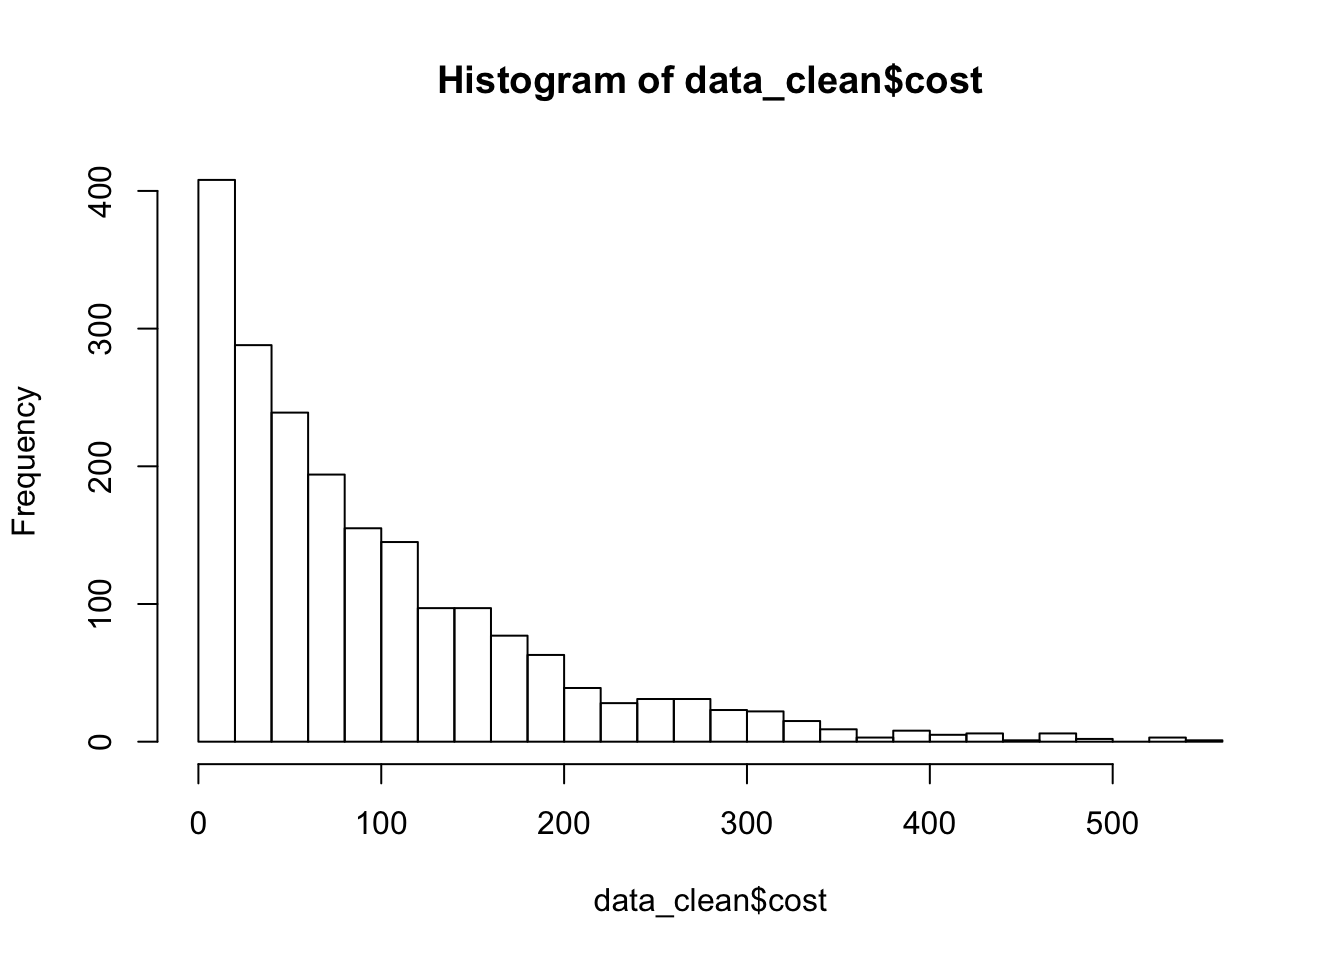
\includegraphics{tp2_files/figure-latex/unnamed-chunk-4-1.pdf}
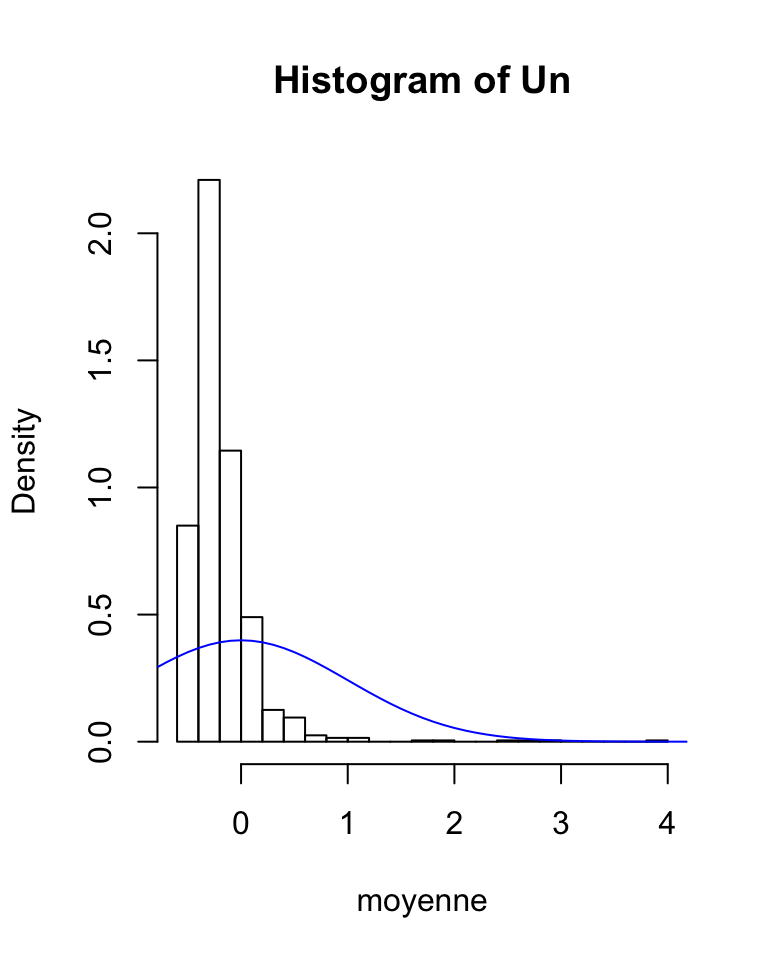
\includegraphics{tp2_files/figure-latex/unnamed-chunk-4-2.pdf}
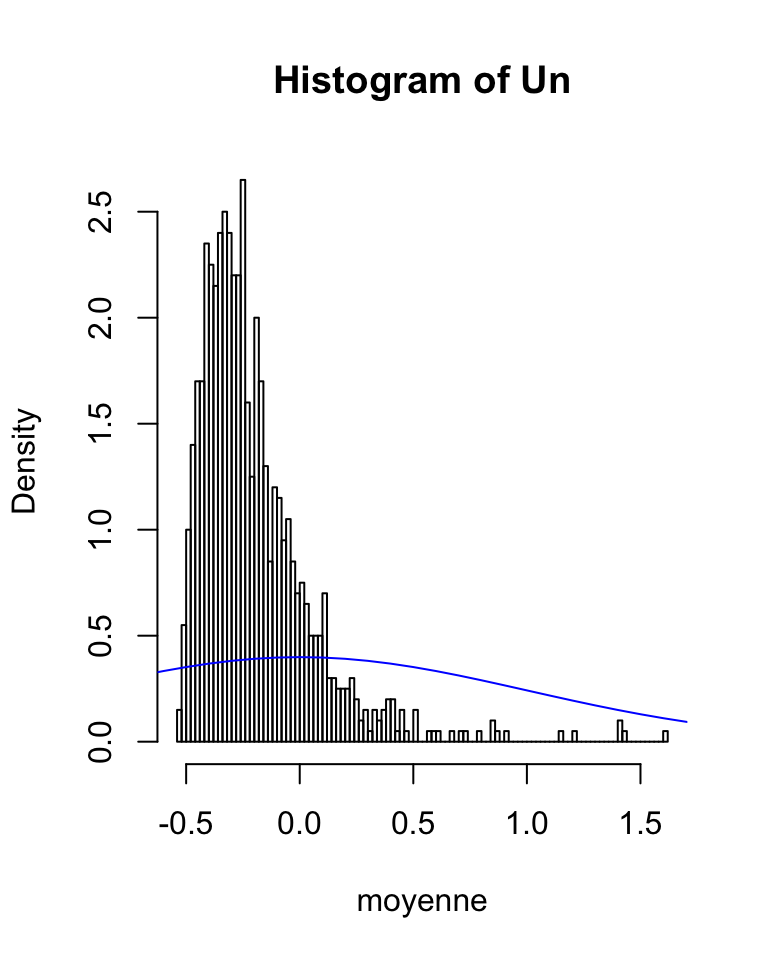
\includegraphics{tp2_files/figure-latex/unnamed-chunk-4-3.pdf}

\begin{Shaded}
\begin{Highlighting}[]
\CommentTok{#hist_moy(function(n)\{return (rnorm(n,mean=1,sd=2))\},"Distribution Gausienne N(1,2)")}
\CommentTok{#moy_norm_hist(function(n) rpareto(n,1,2.5),"AAA")}
\CommentTok{#hist_mul(n)}

\NormalTok{moy_norm_pareto <-}\StringTok{ }\ControlFlowTok{function}\NormalTok{(n,N,a,alpha)\{}
\NormalTok{  Xn <-}\StringTok{ }\KeywordTok{gen_echan_pareto}\NormalTok{(n,N,a,alpha)[}\DecValTok{1}\NormalTok{,]}
\NormalTok{  Un <-}\StringTok{ }\KeywordTok{c}\NormalTok{()}
  \CommentTok{#an <- mean(Xn) }
  \CommentTok{#bn <-sqrt(sd(Xn))}
\NormalTok{  an <-}\StringTok{ }\NormalTok{alpha}\OperatorTok{*}\NormalTok{a}\OperatorTok{/}\NormalTok{(alpha}\DecValTok{-1}\NormalTok{)}
\NormalTok{  bn <-}\StringTok{ }\NormalTok{(alpha}\OperatorTok{*}\NormalTok{a)}\OperatorTok{/}\NormalTok{(alpha}\DecValTok{-1}\NormalTok{)}\OperatorTok{*}\KeywordTok{sqrt}\NormalTok{(alpha}\OperatorTok{/}\NormalTok{(alpha}\DecValTok{-2}\NormalTok{))}\OperatorTok{/}\KeywordTok{sqrt}\NormalTok{(n)}
  \ControlFlowTok{for}\NormalTok{ (i }\ControlFlowTok{in}\NormalTok{ Xn)\{}
    
\NormalTok{    Un <-}\StringTok{ }\KeywordTok{c}\NormalTok{(Un,(i}\OperatorTok{-}\NormalTok{an)}\OperatorTok{/}\NormalTok{bn)}
\NormalTok{  \}}
  \KeywordTok{return}\NormalTok{(Un)}
\NormalTok{\}}

\KeywordTok{hist}\NormalTok{(}\KeywordTok{moy_norm_pareto}\NormalTok{(}\DecValTok{100}\NormalTok{,}\DecValTok{1000}\NormalTok{,}\FloatTok{1.0}\NormalTok{,}\DecValTok{3}\NormalTok{),}\DataTypeTok{breaks=}\DecValTok{100}\NormalTok{)}
\end{Highlighting}
\end{Shaded}

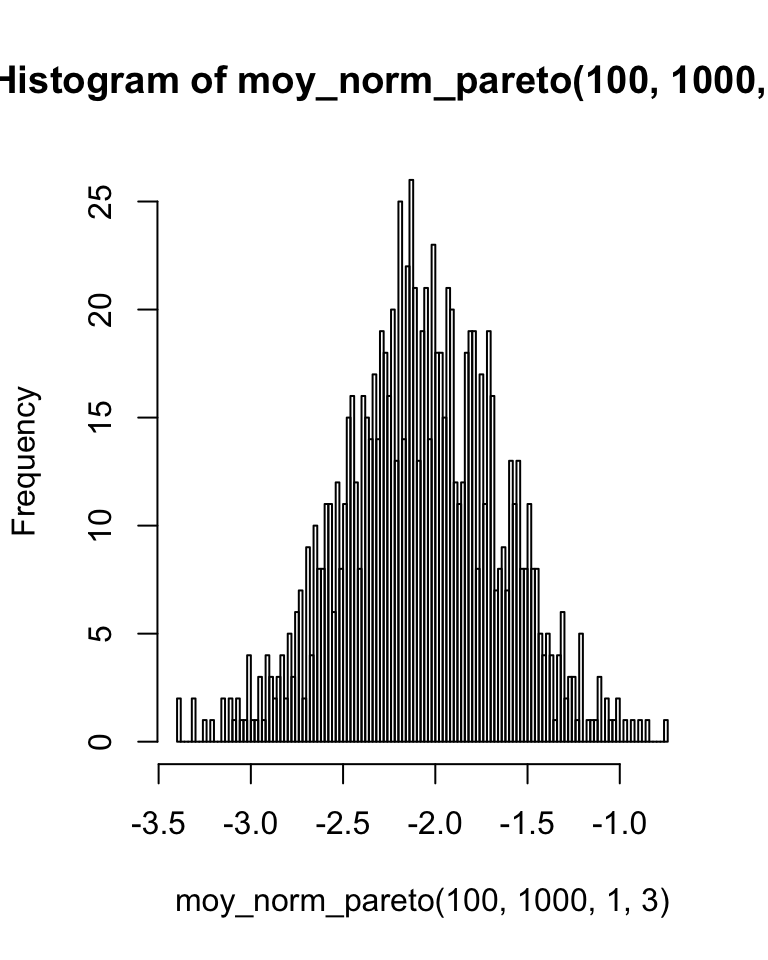
\includegraphics{tp2_files/figure-latex/unnamed-chunk-4-4.pdf}

\#\#\#1.3 Loi de Poisson

Soit X une variable aléatoire suivant une loi de Poisson qu'on notera
\(\mathcal{P}(\lambda)\). Alors, \(\mathbb{E}[X]=\lambda\) et
\(\mathbb{V}[X]=\lambda\) On cherche de nouveau à impliquer le théorème
centrale limite : On a alors rapidement : \(a_n=\lambda\) et
\(b_n=\sqrt{\frac{\lambda}{n}}\)

Comme pour les questions précédentes, on remarque que plus n est grand,
plus la loi moyenne empirique normalisé semble suivre une loi N(0, 1).

\begin{Shaded}
\begin{Highlighting}[]
\NormalTok{gen_echan_poisson <-}\StringTok{ }\ControlFlowTok{function}\NormalTok{(n,N,lambda)\{}
\NormalTok{    x <-}\StringTok{ }\KeywordTok{rpois}\NormalTok{(n,lambda)}
\NormalTok{    aleatoire <-}\StringTok{ }\ControlFlowTok{function}\NormalTok{(x1,n1)\{}
\NormalTok{      y <-}\StringTok{ }\KeywordTok{sample}\NormalTok{(x1,n1,}\DataTypeTok{replace=}\OtherTok{TRUE}\NormalTok{)}
\NormalTok{      moy_sd <-}\StringTok{ }\KeywordTok{c}\NormalTok{(}\KeywordTok{mean}\NormalTok{(y),}\KeywordTok{sd}\NormalTok{(y))}
     \KeywordTok{return}\NormalTok{(moy_sd)}
\NormalTok{    \}}
\NormalTok{  result <-}\StringTok{ }\KeywordTok{sapply}\NormalTok{(}\DecValTok{1}\OperatorTok{:}\NormalTok{N,}\ControlFlowTok{function}\NormalTok{(w) }\KeywordTok{aleatoire}\NormalTok{(x,n))}
  
  \KeywordTok{return}\NormalTok{(result)}
\NormalTok{\}}

\NormalTok{hist_mul <-}\StringTok{ }\ControlFlowTok{function}\NormalTok{(n)\{}
  \ControlFlowTok{for}\NormalTok{ (i }\ControlFlowTok{in}\NormalTok{ n)\{}
    \KeywordTok{hist}\NormalTok{(}\KeywordTok{gen_echan_poisson}\NormalTok{(i,N,}\DecValTok{1}\NormalTok{)[}\DecValTok{1}\NormalTok{,],}\DataTypeTok{breaks=}\NormalTok{i)}
\NormalTok{    t <-}\StringTok{ }\KeywordTok{seq}\NormalTok{(}\OperatorTok{-}\DecValTok{10}\NormalTok{,}\DecValTok{10}\NormalTok{,}\DataTypeTok{by=}\FloatTok{0.5}\NormalTok{)}
\NormalTok{x <-}\StringTok{ }\KeywordTok{dnorm}\NormalTok{(t,}\DecValTok{1}\NormalTok{,}\DecValTok{2}\NormalTok{)}
\KeywordTok{par}\NormalTok{(}\DataTypeTok{new=}\OtherTok{TRUE}\NormalTok{)}
\KeywordTok{plot}\NormalTok{(x)}
\NormalTok{  \}}
\NormalTok{\}}
\CommentTok{#hist_moy(function(n)\{return (rnorm(n,mean=1,sd=2))\},"Distribution Gausienne N(1,2)")}
\CommentTok{#hist_mul(n)}
\NormalTok{gen_echan_law_norm <-}\StringTok{ }\ControlFlowTok{function}\NormalTok{(law,lambda)\{}
  \ControlFlowTok{for}\NormalTok{ (i }\ControlFlowTok{in}\NormalTok{ n)\{}
\NormalTok{    SampleMeans <-}\StringTok{ }\KeywordTok{sapply}\NormalTok{(}\DecValTok{1}\OperatorTok{:}\NormalTok{N,}\ControlFlowTok{function}\NormalTok{(w) }\KeywordTok{moy_empirique}\NormalTok{(}\KeywordTok{sample}\NormalTok{(}\KeywordTok{law}\NormalTok{(i),n,}\DataTypeTok{replace=}\OtherTok{TRUE}\NormalTok{)))}
\NormalTok{    Un <-}\KeywordTok{c}\NormalTok{()}
\NormalTok{    an <-}\StringTok{ }\NormalTok{lambda}
\NormalTok{    bn <-}\StringTok{ }\NormalTok{lambda}\OperatorTok{/}\KeywordTok{sqrt}\NormalTok{(i)}
\NormalTok{    Un <-}\StringTok{ }\NormalTok{(SampleMeans }\OperatorTok{-}\StringTok{ }\NormalTok{an)}\OperatorTok{/}\NormalTok{bn }
    \KeywordTok{hist}\NormalTok{(Un,}\DataTypeTok{prob=}\OtherTok{TRUE}\NormalTok{,}\DataTypeTok{xlab=}\StringTok{"moyenne"}\NormalTok{,}\DataTypeTok{breaks=}\NormalTok{i)}
    \KeywordTok{curve}\NormalTok{(}\KeywordTok{dnorm}\NormalTok{(x,}\DecValTok{0}\NormalTok{,}\DecValTok{1}\NormalTok{),}\DataTypeTok{add=}\OtherTok{TRUE}\NormalTok{,}\DataTypeTok{col=}\StringTok{"blue"}\NormalTok{,}\OperatorTok{-}\DecValTok{5}\NormalTok{,}\DecValTok{5}\NormalTok{)}
\NormalTok{  \}}
\NormalTok{\}}

\KeywordTok{gen_echan_law_norm}\NormalTok{(}\ControlFlowTok{function}\NormalTok{(n) \{}\KeywordTok{return}\NormalTok{ (}\KeywordTok{rpois}\NormalTok{(n,}\DecValTok{3}\NormalTok{))\},}\DecValTok{3}\NormalTok{)}
\end{Highlighting}
\end{Shaded}

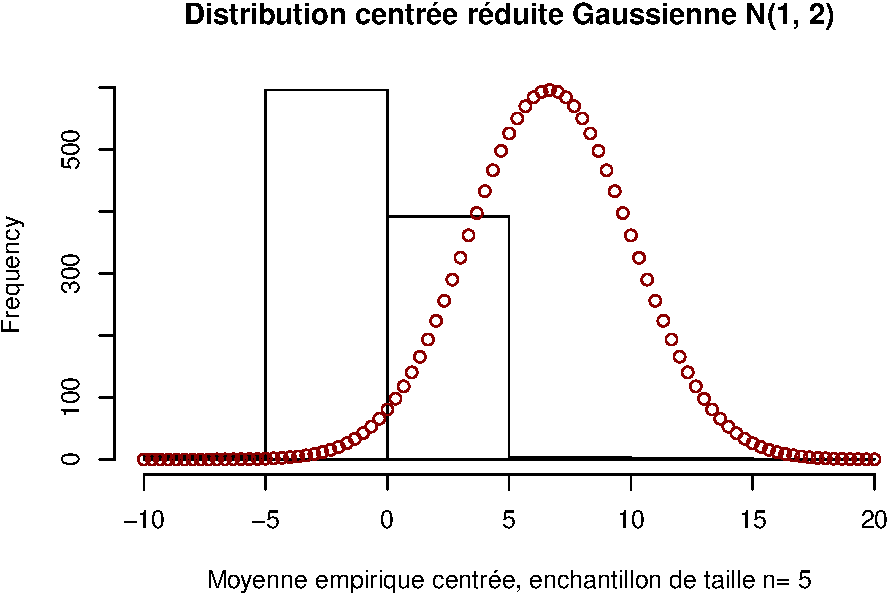
\includegraphics{tp2_files/figure-latex/unnamed-chunk-5-1.pdf}
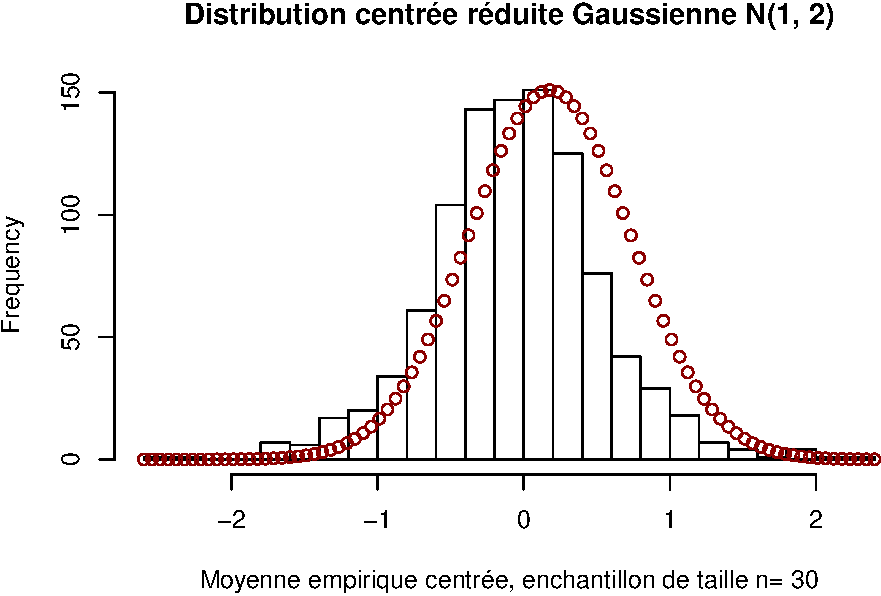
\includegraphics{tp2_files/figure-latex/unnamed-chunk-5-2.pdf}
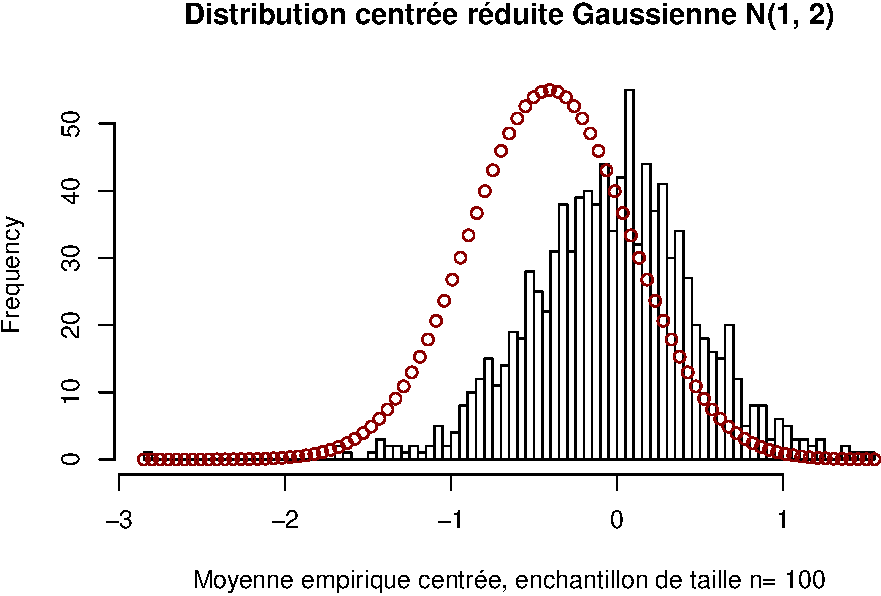
\includegraphics{tp2_files/figure-latex/unnamed-chunk-5-3.pdf}

\begin{Shaded}
\begin{Highlighting}[]
\NormalTok{moy_norm_poisson <-}\StringTok{ }\ControlFlowTok{function}\NormalTok{(n,N,lambda)\{}
\NormalTok{  Xn <-}\StringTok{ }\KeywordTok{gen_echan_poisson}\NormalTok{(n,N,lambda)[}\DecValTok{1}\NormalTok{,]}
\NormalTok{  Un <-}\StringTok{ }\KeywordTok{c}\NormalTok{()}
\NormalTok{  an <-}\StringTok{ }\KeywordTok{mean}\NormalTok{(Xn)}
\NormalTok{  bn <-}\StringTok{ }\KeywordTok{sqrt}\NormalTok{(}\KeywordTok{sd}\NormalTok{(}\KeywordTok{gen_echan_poisson}\NormalTok{(n,N,lambda)[,}\DecValTok{1}\NormalTok{]))}
  \ControlFlowTok{for}\NormalTok{ (i }\ControlFlowTok{in}\NormalTok{ Xn)\{}
    
\NormalTok{    Un <-}\StringTok{ }\KeywordTok{c}\NormalTok{(Un,(i}\OperatorTok{-}\NormalTok{an)}\OperatorTok{/}\NormalTok{bn)}
\NormalTok{  \}}
  \KeywordTok{return}\NormalTok{(Un)}
\NormalTok{\}}

\CommentTok{#hist(moy_norm_poisson(100,1000,1),breaks=100)}
\end{Highlighting}
\end{Shaded}

\#\#\#1.4 Méthodologie d'estimation

Soit \(X=(X_1, ..., X_n)\), où \(n \in \mathbb{R}\), un échantillon. De
plus, on suppose que tous les \(X_{i}\) son i.i.d de même loi.

Soit \(T : \Omega^n \rightarrow \mathbb{R}\) statistique sur un
echantillon de taille n.

Pour trouver une approximation, on fait : 1. Soit \(N \in \mathbb{N}\)
tq \(N \gg 1\) et soit \(N\) échantillons de taille n, notés
\(X^i = (X^i_1, ..., X^i_n)\) tel que \(1 \leq i \leq N\) On introduit
:\$ T\_\{N\} =
\frac{1}{N}\sum\limits\_\{i=1\}\textsuperscript{\{N\}\{T(X}\{i\})\} \$
D'après le théorème centrale limite, on en déduit que lorsque N devient
grand alors: D'une part, on a :
\(\mathbb{E}[ T_N] \xrightarrow[N \gg 1]{} \mathbb{E}[T(X)]\) et,
d'autre part, on a aussi :
\(\mathbb{V}[ T_N] \xrightarrow[N \gg 1]{} \frac{1}{N}\mathbb{V}[T(X)] \xrightarrow[N \rightarrow +\infty]{} 0\)
Avec ce qui précéde, on a finalement \$
T\_n\{\xrightarrow[N \rightarrow +\infty]{\mathbb {L} ^{2}}
\mathbb{E}{[}T(X){]} = c\^{}\{te\}\}\$.

N influence a qualité de l'approximation dans le sens où, comme observé
dans les précédentes question, plus il est grand plus celle-ci est de
bonne qualité.

\#2. Moyenne et dispersion

\#\#\#2.1 Inégalité de Tchebytchev

On considère une variable aléatoire X qui admet un moment d'ordre 2. On
a alors l'inégalité bien connu :
\[\forall \delta > 0, \mathbb{P}(|X-\mathbb{E}[X]|\geq\delta)<\frac{\mathbb{V}[X]}{\delta^{2}}\]

Dans le cas d'une loi Gaussienne, on a alors :
\[\forall \delta > 0, \mathbb{P}(|X-\mu|\geq \delta)<\frac{\sigma^{2}}{\delta^{2}}\]
Dans le cas d'une loi de Poisson, c'est :
\[\forall \delta >0, \mathbb{P}(|X-\lambda|\geq \delta)<\frac{\lambda}{\delta^{2}}\]

\#\#\#2.2 Monte-Carlo \#\#\#\#2.2.1 On a immédiatement que
\[\mathbb{P}(|X-\mu|\geq\delta)=\mathbb{E}[\mathbb{1}_{|X-\mu|\geq\delta}]\]
On pose alors \[Z=1_{|X-\mu|\geq\delta}\]

\#\#\#\#2.2.2

Par hypothèse N est supposé grand, on peut alors en réutilisant les
conclusion de la partie 1, estimer \(\mathbb{E}[Z]\) par la moyenne
empirique : \[Z_{n}= \frac{1}{n}\sum\limits_{i=1}^{n}T(Z^{i})\]


\end{document}
